\documentclass{VUMIFPSkursinis}
\usepackage{algorithmicx}
\usepackage{algorithm}
\usepackage{algpseudocode}
\usepackage{amsfonts}
\usepackage{amsmath}
\usepackage{bm}
\usepackage{caption}
\usepackage{color}
\usepackage{float}
\usepackage{graphicx}
\usepackage{listings}
\usepackage{subfig}
\usepackage{wrapfig}
\usepackage{sectsty}
\usepackage{enumerate}

\usepackage{enumitem}
%PAKEISTA, tarpai tarp sąrašo elementų
\setitemize{noitemsep,topsep=0pt,parsep=0pt,partopsep=0pt}
\setenumerate{noitemsep,topsep=0pt,parsep=0pt,partopsep=0pt}
\allsectionsfont{\centering}
% Titulinio aprašas
\university{Vilniaus universitetas}
\faculty{Matematikos ir informatikos fakultetas}
\department{Programų sistemų katedra}
\papertype{Programų sistemų inžinerijos II laboratorinis darbas}
\title{Socialinis Vilniaus universiteto tinklalapis}
\titleineng{SocialVU}
\status{2 kurso 4 grupės studentai}
\author{Andrejus Voitovas}
\secondauthor{Eglė Puodžiūnaitė}
\thirdauthor{Kasparas Kralikas}
\fourthauthor{Ieva Vizgirdaitė} % Pridėti antrą autorių
\supervisor{asist. dr. Vytautas Valaitis}
\date{Vilnius – \the\year}

% Nustatymai
% \setmainfont{Palemonas}   % Pakeisti teksto šriftą į Palemonas (turi būti įdiegtas sistemoje)
\bibliography{bibliografija}

\begin{document}
% PAKEISTA
\maketitle
\cleardoublepage\pagenumbering{arabic}
\setcounter{page}{2}
\sectionnonum{ANOTACIJA}
IEVA/KASPARAS
\newpage
%TURINYS
\tableofcontents
\sectionnonum{ĮVADAS}
IEVA/KASPARAS
\newpage

\section{FUNKCINIAI REIKALAVIMAI}
Šiame skyriuje pateikiami funkciniai reikalavimai – nagrinėjami scenarijai, ką sistema turi daryti, kaip elgtis vienu ar kitu atveju. Apibrėžiant funkcinius reikalavimus naudojamos procesų sekų diagramos, sistemoje vykdomų užduočių diagramos.
\subsection{Internetinės svetainės langai}
\begin{enumerate}[label=FR1.\arabic*] 
	\item Svetainės langas „Prisijungimas“ turi būti matomas visiems net ir neprisijungusiems naudotojams.
	\item Svetainės langai „Pagrindinis puslapis“, „Dėstytojai“, „Dėstytojo puslapis“, „D.U.K.“, „Renginiai“, „Žinutės“, „Mano profilis“, „Renginio informacija“ turi būti matomi visiems prisijungusiems naudotojams.
	\item Svetainės langas „Konspektai“ turi būti matomas visiems prisijungusiems studentams bei sistemos adminstratoriams.
	\item Svetainės langas „Dėstytojo puslapio redagavimas“ turi būti matomas visiems prisijungusiam puslapį sukūrusiam dėstytojui.
\end{enumerate}
\subsection{Prisijungimas}
\begin{enumerate}[label=FR2.\arabic*] 
	\item Naudotojui suvedus tinkamus prisijungimo duomenis jis turi būti prijungiamas prie sistemos.
	\item Naudotojui netinkamai įvedus prisijungimo duomenis jis neturi būti prijungiamas prie sistemos ir turi būti išmetamas klaidos pranešimas.
	\item Turi būti galimybė užmiršus slaptažodį gautį naują slaptažodį į el. paštą.
	\item Naudotojų bandymų prisijungti prie sistemos skaičius neturi būti ribojamas.\newline
\end{enumerate}

\ref{fig:login} pav. pateikiama užduoties „Prisijungimas” sekų diagrama. Joje vaizduojamas pagrindinis prisijungimo prie sistemos scenarijus ir taip pat nagrinėjami alternatyvūs scenarijai.
\begin{figure}[H]
	\centering
	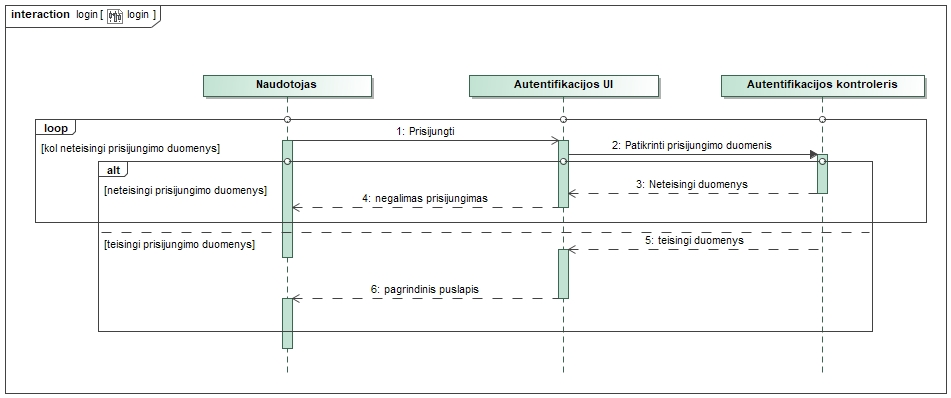
\includegraphics[width=\linewidth]{img/login.jpg}
	\caption{Proceso „Prisijungimas“ sekų diagrama}
	\label{fig:login}
\end{figure}

\subsection{Atsijungimas}
\begin{enumerate}[label=FR3.\arabic*] 
	\item Naudotojas paspaudęs mygtuką atsijungti turi būti atjungiamas
	nuo sistemos.
	\item Atsijungus nuo sistemos ir bandant paspausti grįžimo mygtuką naudotojas turi būti nukreipiamas į prisijungimo langą.
\end{enumerate}
\subsection{Paskyros valdymas}
\begin{enumerate}[label=FR4.\arabic*] 
	\item Naudotojui paspaudus mygtuką „Mano profilis“ turi būti matoma visa žinoma informacija apie naudotoją.
	\item Naudotojui paspaudus mygtuką „Pakeisti slaptažodį“,
	įvedus tinkamą seną ir naują slaptažodžius bei paspaudus
	mygtuką „Patvirtinti“ slaptažodis turi būti pakeičiamas į naują.
	\item Naudotojui paspaudus mygtuką „Pakeisti slaptažodį“ ir
	įvedus netinkamą seną slaptažodį turi būti išvedamas klaidos pranešimas.
	\item Naudotojui paspaudus mygtuką „Pakeisti slaptažodį“ ir
	įvedus netinkamo formato naują slaptažodį turi būti išvedamas klaidos pranešimas ir slaptažodis neturi būti pakeičiamas nauju.
\end{enumerate}
\subsection{Naujienos}
\begin{enumerate}[label=FR5.\arabic*] 
	\item Naujienos turi būti matomos pagrindiniame tinklalapio puslapyje.
	\item Visas naujienų sąrašas turi būti pateikiamas viename puslapyje.
	\item Naujienos turi būti rikiuojamos pagal naujienos paskelbimo datą (naujausios turi būti matomos pirmos).
	\item Jei naujienų sąrašas tuščias turi būti rodomas pranešimas,
	kad naujienų šiuo metu nėra.
	\item Naujienos turi būti matomos visiems prisijungusiems naudotojams.
	\item Naujienos redagavimo funkcija turi būti matoma bei panaudojama tik naujieną paskelbusiam naudotojui.
	\item Skelbti naujienas turi būti galimybė tik prisijungusiems dėstytojams bei sistemos administratoriams.
	\item Naujienos ištrynimo funkcija turi būti matoma bei panaudojama tik naujieną paskelbusiam naudotojui bei sistemos administratoriui.\newline
\end{enumerate}

\ref{fig:delnews} pav. pateikiama užduoties „Naujienos ištrynimas” sekų diagrama. Joje vaizduojamas pagrindinis
naujienos ištrynimo scenarijus.
\begin{figure}[H]
	\centering
	\includegraphics[width=\linewidth]{img/deleteNew.png}
	\caption{Proceso „Naujienos ištrynimas“ sekų diagrama}
	\label{fig:delnews}
\end{figure}

\subsection{Renginiai}
\begin{enumerate}[label=FR6.\arabic*] 
	\item Renginiai turi būti matomi puslapyje „Renginiai“.
	\item Visas renginių sąrašas turi būti pateikiamas kalendoriuje esančiame puslapyje „Renginiai“.
	\item Paspaudus ant kalendoriuje pateikto renginio turi atsidaryti puslapis „Renginio informacija“, kuriame renginys turi būti aprašytas detaliau.
	\item Jei nėra sukurta jokių renginiu, puslapyje „Renginiai“ turi būti pateikiamas tuščias kaledorius.
	\item Renginiai turi būti matomi visiems prisijungusiems naudotojams.
	\item Renginio redagavimo funkcija turi būti matoma bei panaudojama tik renginį sukūrusiam naudotojui.
	\item Kurti renginius turi būti galimybė tik prisijungusiems dėstytojams bei sistemos administratoriams.
	\item Renginio ištrynimo funkcija turi būti matoma bei panaudojama tik naujieną paskelbusiam naudotojui bei sistemos administratoriui.\newline
\end{enumerate}

\ref{fig:addevent} pav. pateikiama užduoties „Renginio sukūrimas” sekų diagrama. Joje vaizduojamas pagrindinis
renginio sukūrimo scenarijus.
\begin{figure}[H]
	\centering
	\includegraphics[width=\linewidth]{img/addNewEvent.png}
	\caption{Proceso „Renginio sukūrimas“ sekų diagrama}
	\label{fig:addevent}
\end{figure}

\subsection{D.U.K.}
\begin{enumerate}[label=FR7.\arabic*] 
	\item Dažniausiai užduodami klausimai turi būti matomi puslapyje „D.U.K.“.
	\item Visas dažniausiai užduodamų klausimų sąrašas turi būti pateikiamas viename puslapyje.
	\item Paspaudus ant vieno iš pateiktų klausimų turi būti matomas atsakymas į tą klausimą.
	\item D.U.K. turi būti matomi visiems prisijungusiems naudotojams.
	\item D.U.K. redagavimo funkcija turi būti matoma bei panaudojama tik sistemos administratoriams.
	\item Sukurti naują klausimą turi būti galimybė tik sistemos administratoriams.
	\item Klausimo ištrynimo funkcija turi būti matoma bei panaudojama tik sistemos administratoriui.\newline
\end{enumerate}

\ref{fig:addduk} pav. pateikiama užduoties „D.U.K.pridėjimas” sekų diagrama. Joje vaizduojamas pagrindinis
D.U.K. pridėjimo scenarijus.
\begin{figure}[H]
	\centering
	\includegraphics[width=\linewidth]{img/addDUK.png}
	\caption{Proceso „D.U.K.pridėjimas” sekų diagrama}
	\label{fig:addduk}
\end{figure}

\subsection{Dėstytojų sąrašas}
\begin{enumerate}[label=FR8.\arabic*] 
	\item Dėstytojų sąrašas turi būti matomas puslapyje „Dėstytojai“.
	\item Puslapyje „Dėstytojai“ turi būti paieškos laukas, kurio pagalba galima surasti reikiamą dėstytoją.
	\item Visas dėstytojų sąrašas turi būti pateikiamas viename puslapyje.
	\item Dėstytojai turi būti surikiuoti abecėlės tvarka pagal pavardę ir vardą.
	\item Dėstytojų sąrašas turi būti matomas visiems prisijungusiems naudotojams.
	\item Prie dėstytojo vardo bei pavardės turi būti pateikiamos nuorodos į dėstytojo puslapį bei į žinutės išsiuntimo dėstytojui puslapį.
\end{enumerate}

\subsection{Dėstytojo puslapis}
\begin{enumerate}[label=FR9.\arabic*] 
	\item Dėstytojo puslapis turi būti matomas visiems prisijungusiems naudotojams.
	\item Tik prisijungęs dėstytojas turi galimybę sukurti savo puslapį.
	\item Tik prisijungęs dėstytojas sukūręs savo puslapį turi galimybę jį redaguoti.
	\item Dėstytojo puslapyje turi buti nuoroda, kurią paspaudus turi būti galimybė rašyti žinutę pasirinktam dėstytojui.\newline
\end{enumerate}

\ref{fig:editpage} pav. pateikiama užduoties „Dėstytojo puslapio redagavimas” sekų diagrama. Joje vaizduojamas pagrindinis dėstytojo puslapio redagavimo scenarijus.
\begin{figure}[H]
	\centering
	\includegraphics[width=\linewidth]{img/editPage.png}
	\caption{Proceso „Dėstytojo puslapio redagavimas” sekų diagrama}
	\label{fig:editpage}
\end{figure}

\subsection{Žinutės}
\begin{enumerate}[label=FR10.\arabic*] 
	\item Puslapis „Žinutės“ turi būti matomas visiems prisijungusiems naudotojams.
	\item Puslapyje „Žinutės“ turi būti pateikiamos visos gautos bei išsiųstos žinutės.
	\item Visoms gautoms bei išsiųstoms žinutėms pateikti naudojami puslapiai (viename puslapyje 25 žinutės).
	\item Išsiųsti žinutę turi turėti galimybę visi prisijungę naudotojai.
	\item Dėstytojo puslapyje turi buti nuoroda, kurią paspaudus galima būtų rašyti žinutę pasirinktam dėstytojui.
	\item Paspaudus mygtuką „Išsiųsti žinutę“ turi atsidaryti žinutės rašymo langas, kuriame turi būti galimybė pasirinkti naudotoją, kuriam žinutė bus išsiųsta.
	\item Paspaudus žinutės išsiuntimo patvirtinimo mygtuką, žinutė turi būti nusiųstą naudotojui, kuriam ši žinutė turėjo būti išsiųsta.
	\item Turi būti galimybė išsiųsti žinutę daugiau nei vienam naudotojui vienu metu.
	\item Dėstytojas turi turėti galimybę pasirinkti išsiųsti žinutę visai grupei arba kursui studentų.\newline
\end{enumerate}

\ref{fig:sendmessage} pav. pateikiama užduoties „Žinutės išsiuntimas” sekų diagrama. Joje vaizduojamas pagrindinis žinutės išsiuntimo scenarijus.
\begin{figure}[H]
	\centering
	\includegraphics[width=\linewidth]{img/sendMes.png}
	\caption{Proceso „Žinutės išsiuntimas” sekų diagrama}
	\label{fig:sendmessage}
\end{figure}

\subsection{Konspektai}
\begin{enumerate}[label=FR11.\arabic*] 
	\item Puslapis „Konspektai“ turi būti matomas visiems prisijungusiems studentams bei sistemos administratoriui.
	\item Konspektai turi būti pateikiami šalia dėstomo dalyko pavadinimo, o dėstomi dalykai turi būti surikiuoti abecėlės tvarka.
	\item Puslapyje „Konspektai“ turi būti paieškos laukelis, kuriame turi būti galimybė ieškoti dėstomo dalyko.
	\item Puslapyje „Konspektai“ turi būti pateikiami visi studentų įkelti konspektai.
	\item Įkelti konspektą turi turėti galimybę visi prisijungę studentai.
	\item Paspaudus mygtuką „Įkelti konspektą“ turi atsidaryti failų pasirinkimo langas.
	\item Paspaudus konspekto įkėlimo patvirtinimo mygtuką, konspektas turi atsirasti visų konspektų sąraše.
	\item Įkeliant konspektą turi būti nurodomas dėstomas dalykas.\newline
\end{enumerate}

\ref{fig:summary} pav. pateikiama užduoties „Konspekto įkėlimas” sekų diagrama. Joje vaizduojamas pagrindinis konpekto įkėlimo scenarijus ir taip pat nagrinėjami alternatyvūs scenarijai.
\begin{figure}[H]
	\centering
	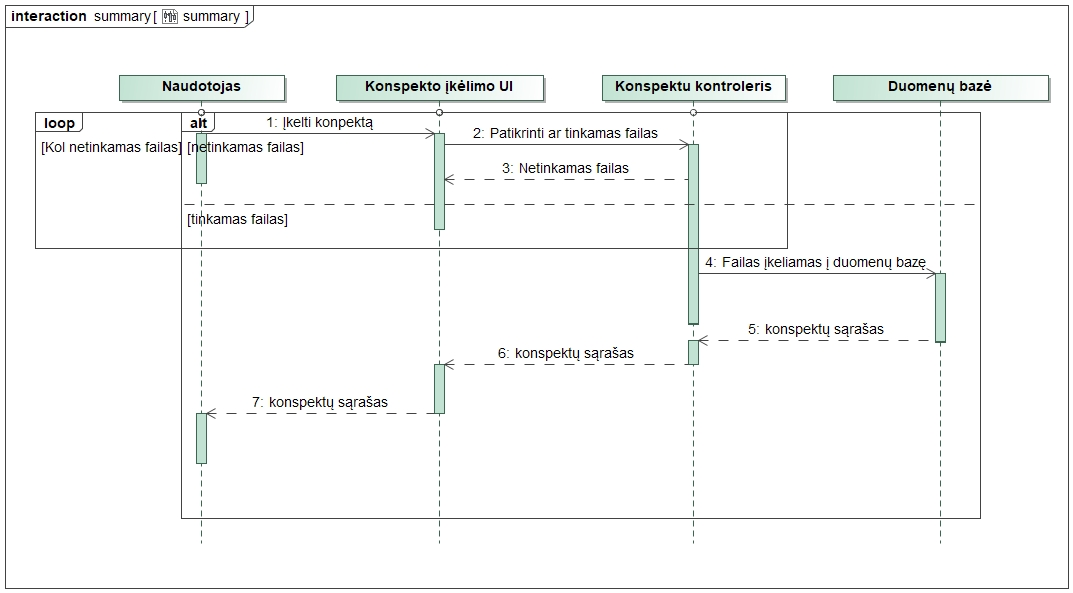
\includegraphics[width=\linewidth]{img/summary.jpg}
	\caption{Proceso „Konspekto įkėlimas“ sekų diagrama}
	\label{fig:summary}
\end{figure}
\newpage

\section{NEFUNKCINIAI REIKALAVIMAI}
ANDRIUS
\newpage

\section{VARTOTOJO SĄSAJOS REIKALAVIMAI}
IEVA/KASPARAS
\newpage

\sectionnonum{IŠVADOS}
IEVA/KASPARAS
\newpage
\end{document}